\DiaryEntry{Inside Interesting Integrals, 2}{2016-02-15}{Maths}

We consider the integral (based on \cite{nahin2020inside}, Section 1.6),

\bee
I = \int_0^\infty \frac{1}{x^3-1} dx
\eee

Apart from the tricky integrand, the integration interval also runs over the singularity of the integrand at $x=1$. Anyway, let's start with a partial fraction expansion (in lack of any other clever ideas anyhow :-)) which yields

\bee
I = \int \frac{1}{3(x-1)} - \frac{x+2}{3(x^2+x+1)}
\eee

The first integral can be solved with the substitution $u = x-1, du/dx = 1$ and therefore

\bee
\int\frac{1}{3}\frac{dx}{x-1} = \frac{1}{3} \int \frac{du}{u} = \frac{1}{3} \ln u = \frac{1}{3} \ln (x-1)
\eee

We will expand the second integrand in one term where the numerator equals the derivative of the denominator, $(x^2+x+1)' = 2x+1$ thus allowing easy substitution, and a ``remaining'' term,

\bee
\frac{x+2}{3(x^2+x+1)} = \frac{1}{3} \frac{1}{2} \frac{2x+4}{x^2+x+1} = \frac{1}{6} \frac{2x+1}{x^2+x+1} - \frac{1}{3}\frac{3}{2}\frac{1}{x^2+x+1} = \frac{1}{6} \frac{2x+1}{x^2+x+1} - \frac{1}{2}\frac{1}{x^2+x+1}
\eee

For the ``remaining'' term we will complete the square to obtain $x^2+x+1 = (x+\frac{1}{2})^2 + \frac{3}{4}$. So we arrive at the following expression for the second integral,

\begin{align*}
  \int \frac{x+2}{3(x^2+x+1)} dx &= \int \frac{1}{6} \frac{2x+1}{x^2+x+1} - \frac{1}{2}\frac{1}{(x+\frac{1}{2})^2 + \frac{3}{4}} dx\\
  &= \frac{1}{6} \int \frac{2x+1}{x^2+x+1} dx - \frac{1}{2} \int \frac{1}{(x+\frac{1}{2})^2 + \frac{3}{4}} dx
\end{align*}

In the first integral we substitute $u = x^2+x+1, du/dx = 2x+1 \rightarrow dx = du/(2x+1)$ and we obtain

\bee
\frac{1}{6} \int \frac{2x+1}{x^2+x+1} dx = \frac{1}{6} \int \frac{2x+1}{u}\frac{du}{2x+1} = \frac{1}{6} \int \frac{du}{u} = \frac{1}{6} \ln u = \frac{1}{6} \ln (x^2+x+1)
\eee

In the second integral we substitute $u = x + \frac{1}{2}, du=dx$ and we get

\bee
\frac{1}{2} \int \frac{1}{(x+\frac{1}{2})^2 + \frac{3}{4}} dx = \frac{1}{2} \int \frac{1}{u^2+\frac{3}{4}} du = \frac{1}{\sqrt{3}} \arctan \frac{2u}{\sqrt{3}} = \frac{1}{\sqrt{3}} \arctan \frac{2 (x+\frac{1}{2})}{\sqrt{3}} = \frac{1}{\sqrt{3}} \arctan \frac{2x+1}{\sqrt{3}}
\eee

Taking everything together, we arrive at the following expression

\bee
I = \frac{1}{3} \ln (x-1) - \frac{1}{6} \ln (x^2+x+1) - \frac{1}{\sqrt{3}} \arctan \frac{2x+1}{\sqrt{3}}
\eee

We can join the first two expressions and arrive at

\bee
\boxed{
  \int_0^\infty \frac{1}{x^3-1} dx = \frac{1}{6} \ln \frac{(x-1)^2}{x^2+x+1} - \frac{1}{\sqrt{3}} \arctan \frac{2x+1}{\sqrt{3}}
  }
\eee

The book then goes to rather great lengths to justify integrating around the singulatory; basically, they consider the limit

\bee
\int_0^\infty \frac{1}{x^3-1} dx = \lim_{\epsilon \rightarrow 0} \left( \int_0^{1-\epsilon} \frac{1}{x^3-1} dx + \int_{1+\epsilon}^\infty \frac{1}{x^3-1} dx \right) \qed
\eee

A similar integral is the following

\bee
I = \int_0^8 \frac{dx}{x-2}
\eee

which has a singularity at $x = 2$. The integrand is shown in the following Figure.


\begin{figure}[H]
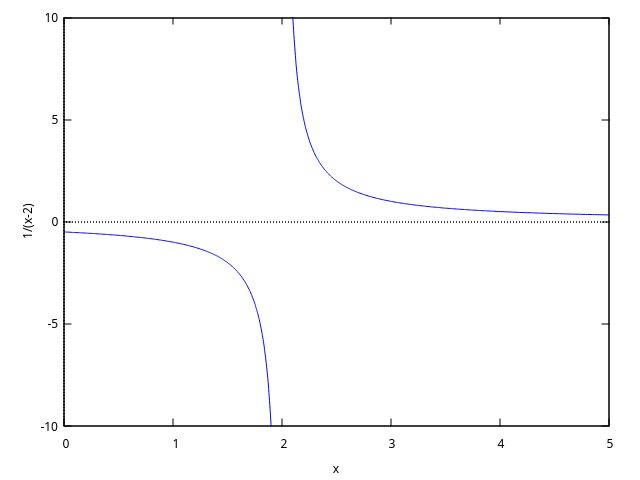
\includegraphics[scale=0.7]{images/2016-02-15_10.png}
\end{figure}

In order to calculate it, we split the integral at the singularity as follows

\bee
I = \lim_{\epsilon \rightarrow 0} \left( \int_0^{2-\epsilon} \frac{dx}{x-2} + \int_{2+\epsilon}^8 \frac{dx}{x-2} \right) = \lim_{\epsilon \rightarrow 0} I_1 + I_2
\eee

For the integrals we make the substitution $u = x-2$ with $du = dx$ and we obtain

\bee
I_1 = \int_0^{2-\epsilon} \frac{dx}{x-2} = \left. \log(x-2) \right|_0^{2-\epsilon} = \log(2 - \epsilon - 2) - \log(-2) = \log(-\epsilon) - \log(-2)
\eee

and

\bee
I_2 = \int_{2+\epsilon}^8 \frac{dx}{x-2} = \left. \log(x-2) \right|{2+\epsilon}^8 = \log(6) - \log(2 + \epsilon - 2) = \log(6) - \log(\epsilon)
\eee

Combining the two results yields

\bee
I_1 + I_2 = \log(-\epsilon) - \log(-2) + \log(6) - \log(\epsilon) = \log \frac{-6\epsilon}{-2\epsilon} = \log \frac{6}{2} = \log(3)
\eee

Interestingly, the $\epsilon$ vanishes; if not,then we would now need to take the limit $\epsilon \rightarrow 0$. We obtain


\bee
\boxed{\int_0^8 \frac{dx}{x-2} = \log(3)}
\eee




%%% Local Variables:
%%% mode: latex
%%% TeX-master: "journal"
%%% End:
